\chapter{บทนำ}

\section{ที่มาและความสำคัญ}


ในช่วงเวลาปัจจุบันนี้ เป็นช่วงที่เกิดปัญหานักศึกษาจบใหม่ว่างงานเพิ่มขึ้นทุกปี \cite{mrgonline} และมีแนวโน้มจะเพิ่มขึ้นอีกเรื่อย ๆ ซึ่งอาจส่งผลให้เกิดความเครียดในหมูนักศึกษาจบใหม่ กระทบการวางแผนชีวิตในอนาคต อาจต้องมีการย้ายสายงาน ทำงานไม่ตรงสายการเรียน เป็นต้น โดยปัญหานี้ เกิดมาจากปัจจัยหลายอย่างทั้งในแง่ระบบการปกครอง ความต้องการของสายอาชีพต่าง ๆ ในตลาดแรงงานที่เปลี่ยนแปลงไป ระบบการศึกษา หรืออื่น ๆ อีกมากมายเกินที่เราจะควบคุมได้ อย่างไรก็ตาม หากเป็นการส่งเสริมด้านการศึกษาเพิ่มเติมด้วยตัวเองและชี้แนะแนวทางนั้น สามารถเป็นไปได้ ทางคณะผู้จัดทำจึงได้เริ่มมองหาจุดที่สามารถเข้าช่วยเหลือและบรรเทาปัญหานี้ โดยเริ่มตั้งเป้าหมายไว้ที่นักศึกษามหาวิทยาลัยเทคโนโลโลยีพระจอมเกล้าธนบุรี คณะวิศวกรรมศาสตร์ สาขาวิศวกรรมคอมพิวเตอร์เป็นกลุ่มแรกก่อน เพื่อนำมาพิสูจน์ผลลัพธ์ของวิธีแก้ปัญหาที่เราออกแบบ

จากการสำรวจกับกลุ่มเป้าหมาย ทางคณะผู้จัดทำได้เล็งเห็นถึงปัญหาบางอย่างร่วมกัน ซึ่งทางคณะผู้จัดทำเองก็ได้ประสบพอเจอด้วยตัวเองตั้งแต่ช่วงชั้นปีที่ 1 และยังคงพบเจออยู่จนถึงปัจจุบันเช่นกัน นั่นคือปัญหาในการค้นหาและเรียนรู้พัฒนาสายอาชีพที่เหมาะสมกับตนเอง ไม่ทราบศาสตร์ความรู้ที่จำเป็นต่อการไปสู่สายงานนั้น ๆ ซึ่งส่งผลโดยตรงไปถึงการเขียนเรซูเมที่อาจไม่ได้สะท้อนถึงองค์ความรู้ที่เหมาะสมกับสายอาชีพมากนัก ทำให้เป็นอุปสรรคต่อการนำไปสมัครงานต่าง ๆ ทั้งการฝึกงานหรืองานเต็มเวลา

จากสิ่งที่กล่าวไป การที่นักศึกษาหลายคนยังไม่สามารถตอบได้เสียด้วยซ้ำว่าตนเองควรพัฒนาตนเองอย่างไร สายอาชีพใดคือสิ่งที่ใช่สำหรับตนเอง แม้จะรู้ว่าต้องการไปต่อในสายงานใดก็ไม่อาจทราบได้ว่าต้องพัฒนาตนเองอย่างไรต่อไปจึงจะตอบโจทย์ตลาดแรงงาน หรือรู้ตัวช้าเกินไปจนพัฒนาได้ไม่ทันการ ซึ่งสะท้อนปัญหาที่ทางคณะผู้จัดเองก็ได้พบเจอด้วย

หากสามารถแก้ไขปัญหานี้ได้ จะช่วยพัฒนาศักยภาพของนักศึกษาได้อย่างรวดเร็วและทำให้พวกขาไปถึงจุดที่ตนเองพอใจได้ง่ายขึ้น เป็นโอกาสที่ดีในการสร้างชื่อให้แก่มหาวิทยาลัย ช่วยให้เห็นแนวทางการพัฒนาตนเองที่ดียิ่งขึ้น และเห็นภาพรวมของสายอาชีพต่าง ๆ

ทางคณะผู้จัดทำจึงมีความสนใจที่จะพัฒนาแพลตฟอร์มสำหรับใช้ช่วยเหลือในการแยกประเภทสายอาชีพที่เหมาะกับเรซูเมนักศึกษากลุ่มเป้าหมายด้วยปัญญาประดิษฐ์ เพื่อให้กลุ่มเป้าหมายได้ทราบแนวทางของเรซูเมของตนเองในปัจจุบัน พร้อมแนะนำแนวทางการไปเรียนรู้ต่อสำหรับนำไปต่อยอดด้วยตนเองได้ เช่น ปรับปรุงให้เหมาะสมกับสายอาชีพที่ต้องการมากขึ้น หรือรับรู้ว่าเรซูเมของตนเองนั้นกำลังอยู่ในทิศทางใด

ดังนั้น  หากคณะผู้จัดทำสามารถใช้โครงงานนี้ในการช่วยเหลือนักศึกษาคนอื่น ๆ ในปัจจุบันหรืออนาคต รวมไปถึงคณะผู้จัดทำเองได้ สิ่งนี้จะเป็นประโยชน์แก่นักศึกษาอย่างยิ่งใหญ่ในด้านการศึกษาและการทำงาน เสมือนเป็นตั๋วเบิกทางให้นักศึกษามหาวิทยาลัยเทคโนโลยีพระจอมเกล้าธนบุรี คณะวิศวกรรมศาสตร์ สาขาวิศวกรรมคอมพิวเตอร์ ในอนาคตหลังจากนี้ ซึ่งเป็นแรงจูงใจที่สำคัญยิ่งกับทางคณะผู้จัดทำที่พบปัญหามาด้วยตนเอง และมีอุดมการณ์อยากช่วยเหลือในด้านนี้เช่นกัน


\section{วัตถุประสงค์}

\begin{itemize}
    \item  เพื่อศึกษาและจับจุดสำคัญของข้อมูลภายในเรซูเมของนักศึกษากลุ่มเป้าหมาย
    \item  เพื่อพัฒนาโมเดลปัญญาประดิษฐ์สำหรับแยกประเภทสายอาชีพที่เหมาะสมจากข้อมูลภายในเรซูเมของนักศึกษาได้
    \item  เพื่อพัฒนาเว็บแอปพลิเคชันสำหรับนำมาใช้เป็นตัวกลางในการใช้งานปัญญาประดิษฐ์ และมีฟีเจอร์เพื่อเป็นตัวช่วยด้านการพัฒนาตนเองและเรซูเมของกลุ่มเป้าหมายได้
    \item  เพื่อพัฒนาประสบการณ์ในการพัฒนาตนเองและช่วยเหลือการปรับปรุงเรซูเม
\end{itemize}


\section{ขอบเขตของโครงงาน}

ขอบเขตด้านเว็บแอปพลิเคชัน
\begin{itemize}
    \item  เว็บแอปพลิเคชันจะมุ่งเน้นสนับสนุนไปที่เพียง 2 ขนาดหน้าจอ คือ เดสก์ท็อปและมือถือ
\end{itemize}

ขอบเขตด้านปัญญาประดิษฐ์
\begin{itemize}
    \item  ผู้ใช้จะต้องกรอกข้อมูลของเรซูเมด้วยตัวเองเพื่อให้ปัญญาประดิษฐ์วิเคราะห์ผลลัพธ์เป็นวิธีหลัก
    \item  ปัญญาประดิษฐ์จะรองรับภาษาอังกฤษในการวิเคราะห์เท่านั้น
\end{itemize}

ขอบเขตด้านเนื้อหาและกลุ่มเป้าหมาย
\begin{itemize}
    \item  มุ่งเน้นไปที่นักศึกษาวิศวกรรมคอมพิวเตอร์หลักสูตรปกติ และนานาชาติ
    \item  สายอาชีพที่สนับสนุนจะประกอบด้วย 6 สายอาชีพดังนี้
    \begin{itemize}
        \item Developer เช่น frontent developer, backend developer และ full-stack developer
        \item Designer เช่น UX/UI Designer
        \item Data และ AI เช่น Data Engineer, Data Science และ Data Analyst
        \item Security เช่น Data Security และ Cyber Security
        \item Cloud Management เช่น DevOps
        \item Quality Assurance และ Tester เช่น Manual/Automate Tester
    \end{itemize}
    เนื่องจากข้อจำกัดจากข้อมูลที่มีในปัญญาประดิษฐ์ ความนิยมของสายอาชีพนั้น ๆ ในตลาดแรงงาน \cite{springnews} และนัยยะสำคัญที่ได้มาจากกลุ่มเป้าหมาย
\end{itemize}

\section{ประโยชน์ที่คาดว่าจะได้รับ}

ทางคณะผู้จัดทำคาดหวังเป็นอย่างยิ่งว่าจะสามารถนำเว็บแอปพลิเคชันนี้มาใช้งานกับนักศึกษาวิศวกรรมคอมพิวเตอร์ทุกชั้นปีซึ่งรวมถึงคณะผู้จัดทำเองด้วย โดยหวังว่าจะช่วยเหลือให้กลุ่มเป้าหมายนี้ สามารถปรังปรุงเรซูเมของตัวเองให้ดียิ่งขึ้น หรือปรับให้เข้ากับความต้องการของตนเอง เสริมความมั่นใจในการนำไปสมัครงานตามช่องทางที่ตนเองสนใจ รวมไปถึงใช้งานเว็บแอปพลิเคชันเพื่อพัฒนาตนเอง อีกทั้งยังสามารถพัฒนาปัญญาประดิษฐ์ให้มีประสิทธิภาพมากขึ้นจากข้อมูลที่ได้รับระหว่างเปิดให้ใช้งานตามเวลาอีกด้วย ซึ่งเป็นประโยชน์อย่างมากในยุคที่ข้อมูลมีความสำคัญเช่นนี้

\section{ตารางการดำเนินงาน}
\begin{figure}[!h]\centering
    \setlength{\fboxrule}{0.2mm}
    \setlength{\fboxsep}{0.5cm}
    \fbox{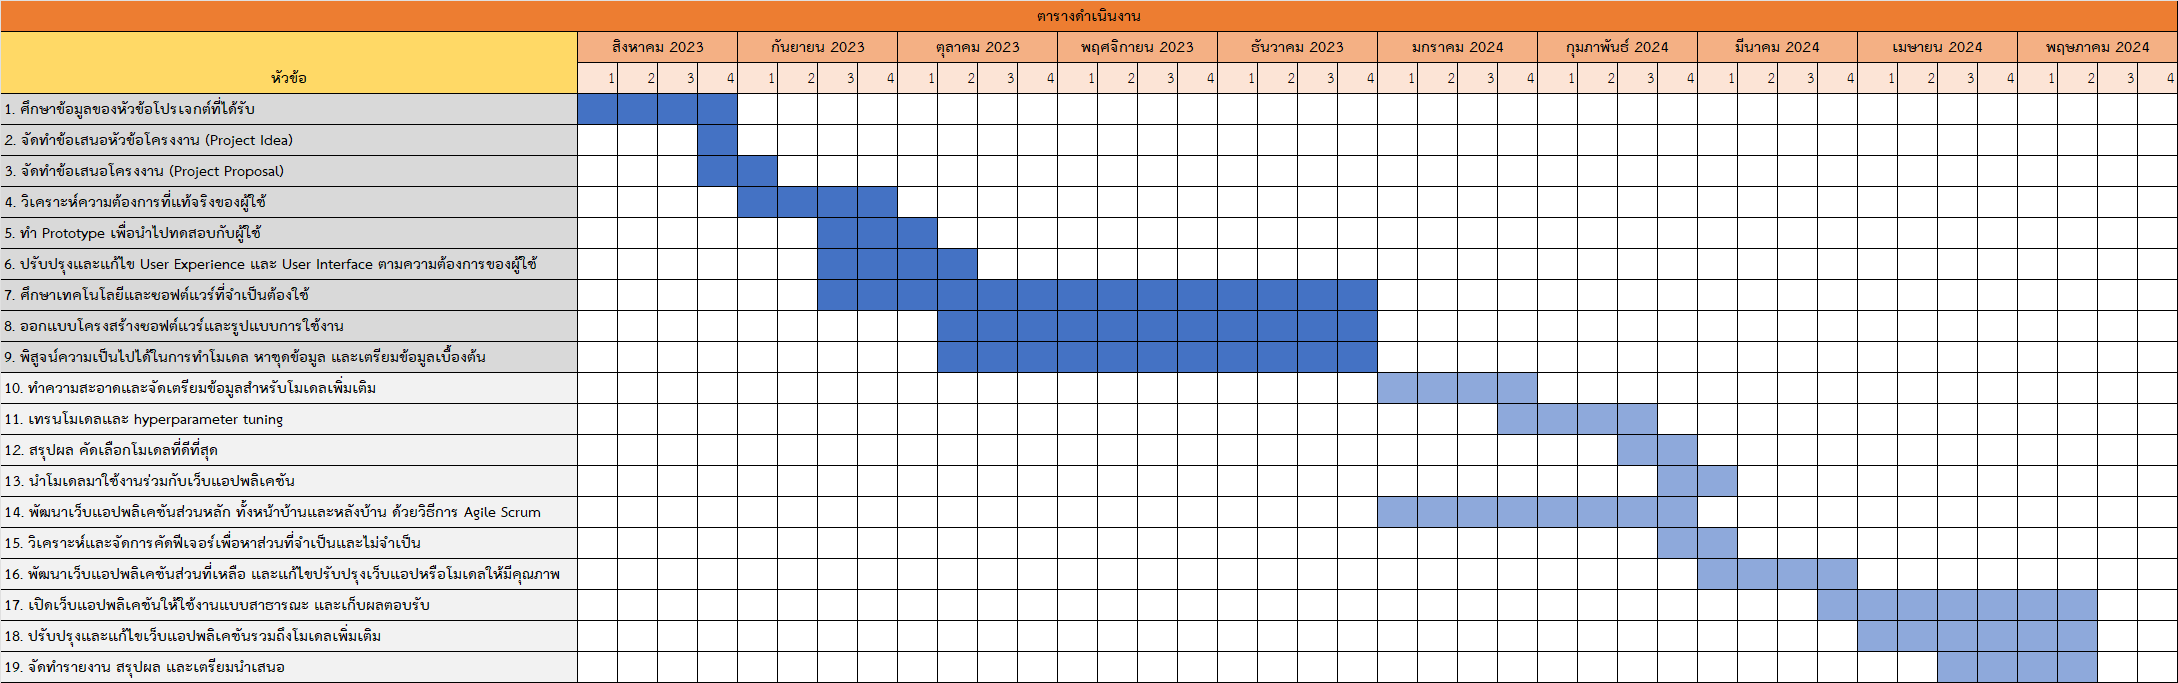
\includegraphics[width=15cm]{./figure/figure_ganttchart.png}}
    \caption{ตารางการดำเนินงาน}\label{fig:grantt chart}
\end{figure}